\documentclass[a4paper]{article}
\usepackage{graphicx}
\usepackage{xcolor}
\usepackage{dirtree}
\usepackage{tikz}
\usetikzlibrary{shapes,arrows}
\newcommand\myicn[1]{{\color{#1}\rule{2ex}{2ex}}}
\newcommand\mydir[3]{{\myicn{#1}\ {\textbf\large#2}:\ {\textnormal{\textit{\color{gray}#3}}}}}

\begin{document}
	\begin{titlepage}
		
\includegraphics[width=0.5\textwidth]{logo.jpg}
		\par
		\centering
		\vspace{1cm}
		{\scshape\LARGE Z\'apado\v{c}esk\'a univerzita v Plzni\\Fakulta aplikovan\'ych v\v{e}d \par}
		\vspace{1cm}
		{\scshape\Huge Dokumentace k semestr\'aln\'i pr\'aci\\KIV/WEB\\Webov\'e str\'anky konferen\v{c}n\'iho
		syst\'emu \par}
		\vspace{1.5cm}
		{\Large\bfseries Martin \v{C}ervenka A14B0239P cervemar@students.zcu.cz \par}
		\vfill
		{\large 2. prosince 2016\par}
	\end{titlepage}
	\section{Pou\v{z}it\'e technologie}
		V aplikaci jsem pou\v{z}il mnoho technologi\'i, mezi ty hlavn\'i \v{r}ad\'im \textit{HTML5}, \textit{CSS},
		\textit{PHP}, \textit{MySQL}, \textit{JavaScript}, \textit{JQuery}, \textit{AJAX}, \textit{Bootstrap},
		\textit{CKEditor} a \textit{htaccess}. N\'asleduje popis t\v{e}chto technologi\'i a m\'ista, kde se tyto
		technologie v aplikaci vyskytuj\'i.
		\begin{itemize}
			\item{\textbf{HTML5}\\}
				Zna\v{c}kovac\'i jazyk HTML5 je z\'akladn\'i technologie, kterou jsem pou\v{z}il.
				Soubory obsahuj\'ic\'i HTML5 lze nal\'est ve slo\v{z}ce \textit{view $\rightarrow$ templates},
				kde je pou\v{z}it i \v{s}ablonovac\'i syst\'em Twig.
			\item{\textbf{CSS}\\}
				Kask\'adov\'e styly jsem pou\v{z}il k drobn\'emu vylep\v{s}en\'i, kdy v\v{e}t\v{s}inu
				styl\r{u} jsem pou\v{z}il z knihovny Bootstrap. P\v{r}\'ikladem souboru kask\'adov\'ych
				styl\r{u} je soubor \textit{style.css} ve slo\v{z}ce \textit{view}.
			\item{\textbf{PHP}\\}
				PHP jsem pou\v{z}il pro zpracov\'an\'i po\v{z}adavk\r{u} od klienta -- jako controller.
				Tyto soubory se nach\'azej\'i ve slo\v{z}ce \textit{controller}. 
			\item{\textbf{MySQL}\\}
				Jako dotazovac\'i jazyk jsem zvolil MySQL. Aplikace ale obsahuje PDO, proto je mo\v{z}n\'e
				dotazovac\'i jazyk pom\v{e}rn\v{e} jednodu\v{s}e zm\v{e}nit. Jako p\v{r}\'iklad uv\'ad\'im
				skript \textit{sql.sql} v ko\v{r}enov\'em adres\'a\v{r}i, nebo soubor \textit{database\_pool.php}
				ve slo\v{z}ce \textit{model}, kter\'y s datab\'az\'i pracuje.
			\item{\textbf{Twig}\\}
				\v{S}ablonovac\'i syst\'em Twig jsem pou\v{z}il zejm\'ena pro zp\v{r}ehledn\v{e}n\'i
				k\'odu. Soubory \v{s}ablon se nach\'azej\'i ve slo\v{z}ce \textit{templates},
				jak jsem ji\v{z} uvedl v\'y\v{s}e v~bod\v{e} 1.
			\item{\textbf{JavaScript, JQuery a AJAX}\\}
				Javascript v kombinaci s JQuery a AJAXem jsem pou\v{z}il hlavn\v{e} pro asynchronn\'i komunikaci
				se serverem. Aplikce v\v{s}ak funguje i pokud m\'a klient javascript deaktivovan\'y -- v tom
				p\v{r}\'ipad\v{e} aplikace komunikuje synchronn\v{e}. Soubory javascriptu se nach\'azej\'i
				ve slo\v{z}ce \textit{controller $\rightarrow$ js}
			\item{\textbf{Bootstrap}\\}
				Pro vzhled aplikace bylo vhodn\'e pou\v{z}\'it knihovnu Bootstrap. Obsahuje mnoho
				p\v{r}edp\v{r}ipraven\'ych styl\r{u} a \v{r}e\v{s}\'i i responzivitu webu.
				Bootstrap je pou\v{z}it ve v\v{e}t\v{s}in\v{e} \v{s}ablon, kter\'e se nach\'azej\'i
				v adres\'a\v{r}i uveden\'em v prvn\'im bod\v{e}.
			\item{\textbf{CKEditor}\\}
				Pro jednodu\v{s}\'i pou\v{z}\'iv\'an\'i aplikace jsem do aplikace p\v{r}idal CKEditor.
				Tato knihovna vytvo\v{r}\'i u\v{z}ivatelsky p\v{r}\'iv\v{e}tiv\'y editor p\v{r}\'imo
				na webov\'e str\'ance. CKEditor je p\v{r}id\'an pomoc\'i javascriptu do \v{s}ablony
				\textit{form.tmpl}.
			\item{\textbf{htaccess}\\}
				Htaccess jsem pou\v{z}il pro povolen\'i tzv ''p\v{e}kn\'ych URL''. Soubor \textit{.htaccess}
				se nach\'az\'i p\v{r}\'imo v ko\v{r}enov\'em adres\'a\v{r}i aplikace.
		\end{itemize}
	\clearpage

	\section{Adres\'a\v{r}ov\'a struktura}

		Adres\'a\v{r}ov\'y strom \ref{tree} popisuje strukturu aplikace. Slo\v{z}ky jsou barevn\v{e} odli\v{s}eny
		od soubor\r{u}, kter\'e jsou pro jednoduchost sdru\v{z}eny, pokud maj\'i stejnou p\v{r}\'iponu.

		\begin{figure}[!ht]
			\dirtree{%
				.1 \mydir{black}{/}{Root directory}.
					.2 \mydir{red}{controller}{Funk\v{c}nost webu}.
						.3 \mydir{red}{js}{Obsajuje javascript(y) odes\'ilan\'e klientovi}.
						.3 \mydir{red}{twig}{Knihovna TWIGu}.
						.3 \mydir{white}{*.php}{Soubory zpracov\'avaj\'ic\'i p\v{r}\'ikazy od klienta}.
					.2 \mydir{blue}{doc}{Soubor(y) dokumetace}.
						.3 \mydir{white}{A14B0239P.pdf}{Tento soubor PDF}.
					.2 \mydir{green}{model}{Data webu}.
						.3 \mydir{white}{*.php}{Soubory pracuj\'ic\'i s daty}.
					.2 \mydir{yellow}{view}{Vzhled webu}.
						.3 \mydir{yellow}{bootstrap}{Knihovna Bootstrapu}.
						.3 \mydir{yellow}{ckeditor}{Knihovna CKEditoru}.
						.3 \mydir{yellow}{templates}{\v{S}ablony TWIGU}.
							.4 \mydir{white}{*.tmpl}{Jednotliv\'e \v{s}ablony TWIGu}.
						.3 \mydir{white}{*.css}{Soubor(y) se styly}.
					.2 \mydir{orange}{texts}{Slo\v{z}ka pro uk\'ad\'an\'i dokument\r{u} PDF od klient\r{u}}.
					.2 \mydir{white}{.htaccess}{Nastaven\'i p\v{r}evodu ''p\v{e}kn\'ych'' URL adres}.
					.2 \mydir{white}{index.php}{Nastavuje TWIG a p\v{r}ed\'av\'a \v{r}\'izen\'i controlleru}.
					.2 \mydir{white}{sql.sql}{Skript pro inicializaci datab\'aze}.
			}
			\caption{Adres\'a\v{r}ov\'a struktura}
			\label{tree}
		\end{figure}
		\clearpage

	\section{Instalace aplikace}
		Instalace aplikace se skl\'ad\'a z n\v{e}kolika krok\r{u}. Na n\v{e}kter\'ych za\v{r}\'izen\'ich
		ji\v{z} m\r{u}\v{z}ou b\'yt prvn\'i t\v{r}i body hotovy, proto je to pot\v{r}eba zkontrolovat.
		
		Pro n\v{e}kter\'e platformy je dostupn\'y bal\'ik (LAMP, XAMP, WAMP, ...), kter\'y spoj\'i prvn\'i t\v{r}i
		body instalace do jednoho bodu. 
		\begin{itemize}
			\item{\textbf{Instalace HTTP serveru}\\}
				Prvn\'im krokem je instalace HTTP serveru. Jedn\'im z nich je server A\-pa\-che.
				Jak takov\'y server nainstalovat lze pro danou platformu naj\'it na internetu.
			\item{\textbf{Instalace PHP}\\}
				Dal\v{s}\'im krokem je instalace PHP. N\'avody na konkr\'etn\'i platformy lze
				op\v{e}t nal\'est na internetu.
			\item{\textbf{Instalace MySQL}\\}
				D\'ale je t\v{r}eba nainstalovat datab\'azov\'y server MySQL. N\'avody na instalaci
				jsou op\v{e}t na internetu.
			\item{\textbf{Vytvo\v{r}en\'i nov\'e datab\'aze}\\}
				Pot\'e je pot\v{r}eba vytvo\v{r}it na datab\'azov\'em serveru pr\'azdnou datab\'azi
				pro tuto aplikaci, jm\'eno je libovoln\'e, stejn\'e se pak nastav\'i v bod\v{e}
				''Nastaven\'i aplikace''.
			\item{\textbf{Spu\v{s}t\v{e}n\'i MySQL skriptu}\\}
				Po vytvo\v{r}en\'i datab\'aze spust\'ime v t\'eto datab\'azi skript sql.sql, kter\'y
				se nach\'az\'i v ko\v{r}enov\'em adres\'a\v{r}i projektu.
			\item{\textbf{Zkop\'irov\'an\'i cel\'eho projektu}\\}
				Pot\'e m\r{u}\v{z}eme cel\'y projekt zkop\'irovat na webov\'y server.
			\item{\textbf{Nastaven\'i aplikace}\\}
				Na \v{r}\'adc\'ich 35 - 38 souboru \textit{model $\rightarrow$ database\_pool.php}
				je pot\v{r}eba nastavit p\v{r}ihla\v{s}ovac\'i \'udaje k datab\'azov\'emu serveru
				a n\'azev datab\'aze. Sta\v{c}\'i p\v{r}epsat defaultn\'i nastaven\'i na t\v{e}chto
				\v{r}\'adc\'ich.
			\item{\textbf{Nastaven\'i pr\'av}\\}
				Slo\v{z}ka \textit{texts} mus\'i m\'it nasten\'e opr\'avn\v{e}n\'i, aby do n\'i mohl
				webov\'y server zapisovat. Pokud tomu tak nen\'i, je pot\v{r}eba to nastavit.
		\end{itemize}

		P\v{r}i spu\v{s}t\v{e}n\'i aplikace neexistuje \v{z}\'adn\'y u\v{z}ivatel, proto prvn\'i vytvo\v{r}en\'y
		dostane nejvy\v{s}\v{s}\'i opr\'avn\v{e}n\'i, dal\v{s}\'i pak b\v{e}\v{z}n\'e opr\'avn\v{e}n\'i.

		\clearpage
	\section{Architektura aplikace}
		Z\'akladn\'i funkcionalitu popisuje diagram \ref{img:diagram}. Cel\'a aplikace funguje dv\v{e}ma zp\r{u}\-so\-by.
		P\v{r}i aktivn\'im javascriptu se nahrazuj\'i asynchronn\v{e} pouze \v{c}\'asti str\'anky, zat\'imco kdy\v{z}
		u\v{z}ivatel javascript deaktivuje, str\'anky se na\v{c}\'itaj\'i cel\'e. To ur\v{c}uje podm\'inka
		\textit{part\_only()}.

		Prvn\'i podm\'inkou v diagramu \ref{img:diagram} je z\'isk\'an\'i parametru z URL. Pokud zde \v{z}\'adn\'y
		parametr nen\'i, pak se nastav\'i parametr \textit{index}.
		\begin{figure}[!ht]	
			\centering
			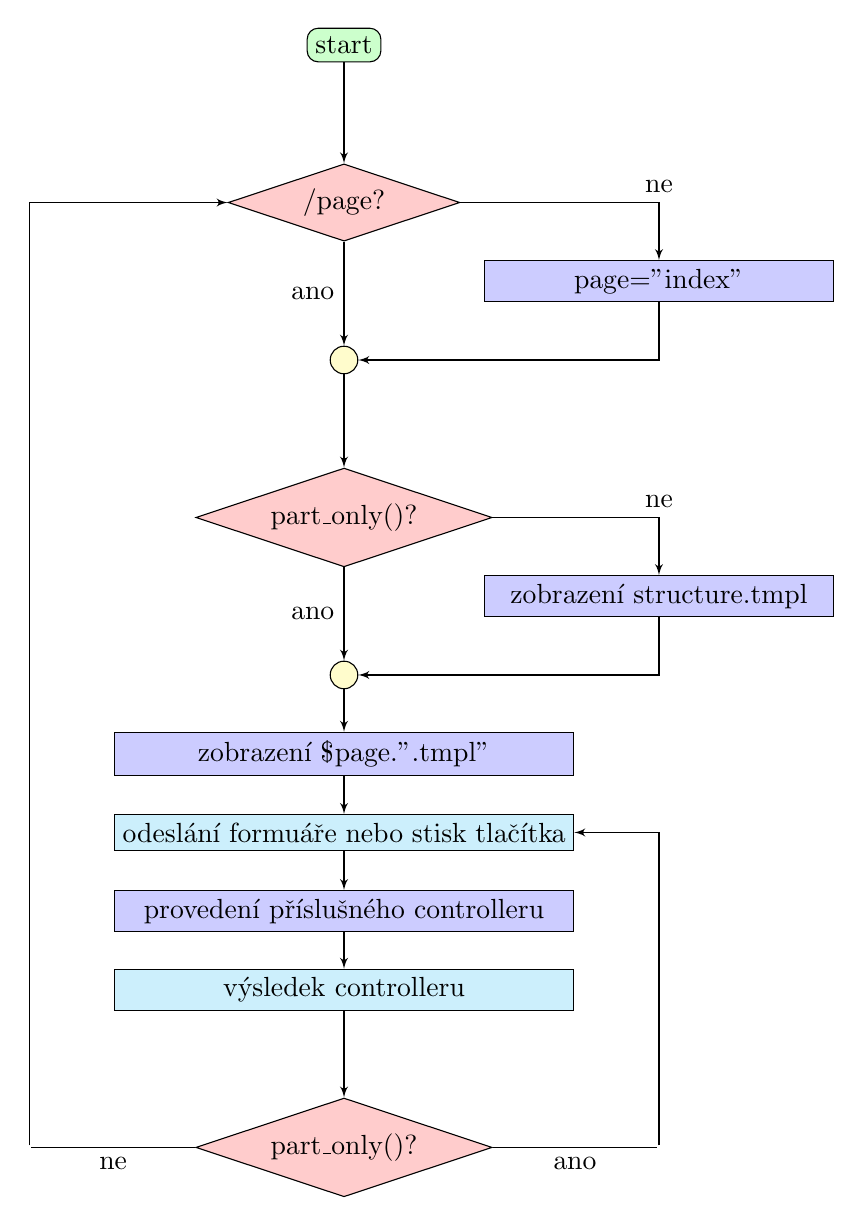
\begin{tikzpicture}
				\tikzstyle{common} = [draw, text badly centered, node distance=1cm and 2cm, inner sep=0.3em]
				\tikzstyle{decision} = [diamond, aspect=3, common, node distance=2cm, fill=red!20]
				\tikzstyle{cloud} = [rectangle, rounded corners, common, fill=green!20]
				\tikzstyle{block} = [rectangle, common, text width=16em, fill=blue!20]	
				\tikzstyle{block2} = [block, fill=cyan!20]
				\tikzstyle{merge} = [circle, common, fill=yellow!20, text width=1em ,inner sep=0]
				\tikzstyle{invisible} = [inner sep=0, draw=none, fill=none]
				\tikzstyle{line} = [draw, -latex']
				\tikzstyle{blockside} = [block, node distance=2cm, text width=12em]
				\node[cloud] (start) {start};
				\node[decision, below of=start] (page) {/page?};
				\node[invisible, below of=page] (i1) {};
				\node[merge, below of=i1] (merge1) {};
				\node[decision, below of=merge1] (part) {part\_only()?};
				\node[invisible, below of=part] (i2) {};
				\node[merge, below of=i2] (merge2) {};
				\node[block, below of=merge2] (pagetmpl) {zobrazen\'i \$page.".tmpl"};
				\node[block2, below of=pagetmpl] (input) {odesl\'an\'i formu\'a\v{r}e nebo stisk tla\v{c}\'itka};
				\node[block, below of=input] (control) {proveden\'i p\v{r}\'islu\v{s}n\'eho controlleru};
				\node[block2, below of=control] (output) {v\'ysledek controlleru};
				\node[decision, below of=output] (po2) {part\_only()?};

				\node[invisible, node distance=4cm, right of=start] (top) {};
				\node[invisible, below of=top] (i3) {};
				\node[blockside, below of=i3] (setpage) {page="index"};
				\node[invisible, below of=setpage] (i4) {};
				\node[invisible, below of=i4] (i5) {};
				\node[blockside, below of=i5] (defpage) {zobrazen\'i structure.tmpl};

				\node[invisible, node distance=4cm, left of=po2] (x1) {};
				\node[invisible, node distance=4cm, right of=po2] (x2) {};
				\draw[line] (start) -- (page);
				\draw[line] (page) -| (setpage) node[midway,above]{ne};
				\draw[line] (page) -- (merge1) node[midway,left]{ano};
				\draw[line] (setpage) |- (merge1);
				\draw[line] (merge1) -- (part);
				\draw[line] (part) -| (defpage) node[midway,above]{ne};
				\draw[line] (part) -- (merge2) node[midway,left]{ano};
				\draw[line] (defpage) |- (merge2);
				\draw[line] (merge2) -- (pagetmpl);
				\draw[line] (pagetmpl) -- (input);
				\draw[line] (input) -- (control);
				\draw[line] (control) -- (output);
				\draw[line] (output) -- (po2);
				\draw[draw] (po2) -- (x1) node[midway,below]{ne};
				\draw[line] (x1) |- (page);
				\draw[draw] (po2) -- (x2) node[midway,below]{ano};
				\draw[line] (x2) |- (input);
			\end{tikzpicture}
			\caption{V\'yvojov\'y diagram}
			\label{img:diagram}
		\end{figure}
\end{document}
